%!TEX root = ../thesis.tex
前提として,開発するロボットアームは,オフィスロボットとして適している必要がある.オフィスロボットとして適した仕様を決定するにあたり,本研究では以下の手順を踏んだ.
\begin{enumerate}
  \item 既存オフィスロボットが対象としている作業の調査
  \item 行う作業の決定
  \item 既存オフィスロボットのロボットアームのメカニズム調査
  \item 仕様の決定
\end{enumerate}
まず,「調査した全てのオフィスロボットが行える作業」を基準に作業を決定し,その作業から求められる項目を,ロボットアーム調査の結果を踏まえて整理した.本章では,本研究で対象とする作業の決定過程と,要求仕様の決定について述べる.

\section{作業調査}
開発するロボットアームが対象とする作業を決定するため,既存のオフィスロボットが対象としている作業を調査した.動画や文献をから合計77件の作業事例を抽出したところ,約61\%が台車移動とピック\&プレイスを組み合わせた作業であった.これは,部屋の片づけや荷物の運搬などが代表例である.それ他の作業としては,ドアの開閉,ボタンの押下,フロアの巡回,などが挙げられた.以上の結果から,現在オフィスロボットが対象としている作業の多くは,物体を把持して移動させる作業であると考えられる.本研究で開発するロボットアームは,将来的にオフィスロボットの標準プラットフォームとして活用されることを目指している.その第一歩として,本研究では「机の片づけ作業」を対象とした.

\section{机の片づけ作業}
ここでは,「机の片づけ作業」の詳細を述べる.机の片づけ作業は,机の上に散らばっている物体を事前に設置した箱の中へ移動させる作業である.以下に,具体的に使用する物体の種類や重量,設置位置について以下に述べる.
\subsection{机の上に置く物体}
机の上に置く物体,すなわちロボットが把持対象とする物体は,既存のオフィスロボットが頻繁に把持していた対象を調査したうえで設定した.図\ref{fig:handget}に示すように,最も多かったのは服やタオルなどの衣類で,次にペットボトルや缶ジュースなどの筒状物,お菓子の箱や 200ml 程度のパックジュースなどの箱状物,さらにペンなどの棒状物や雑誌などの薄型物が続いた.以上の結果に基づき,本研究では作業対象としてタオル,缶ジュース,パックジュースの 3 種類を採用する.
\begin{figure}[h]
  \centering
  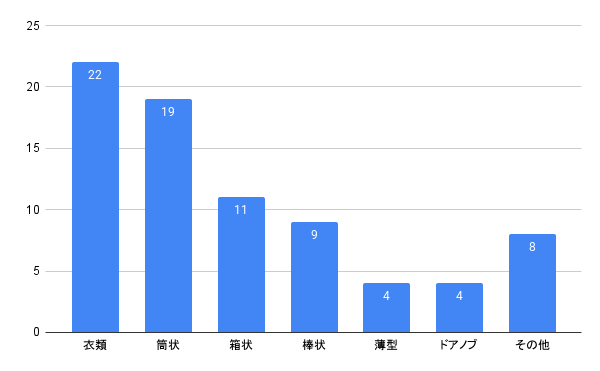
\includegraphics[width=10cm]{images/2syou/handget.png}
  \caption{Survey results of objects grasped by office robots}
  \label{fig:handget}
\end{figure}
\clearpage
\subsection{物体の重量}
調査の中では,人が片手で持てないサイズや重量の大きい物体を扱う事例は見られなかった.そこで,把持対象物の重量は 500g 以下と設定した.
\subsection{物体の設置位置}
次節で詳述するように,既存のオフィスロボットのアームリーチで最小の値は,Hello Robot 社が開発している Stretch 3 の約 0.51m であった.したがって,把持対象物と箱の設置位置は,机の縁から0.5m以内の範囲に設置することとする.
\newpage